%-----------------------------------LICENSE------------------------------------%
%   This file is part of tikz_figures.                                         %
%                                                                              %
%   tikz_figures is free software: you can redistribute it and/or              %
%   modify it it under the terms of the GNU General Public License as          %
%   published by the Free Software Foundation, either version 3 of the         %
%   License, or (at your option) any later version.                            %
%                                                                              %
%   tikz_figures is distributed in the hope that it will be useful,            %
%   but WITHOUT ANY WARRANTY; without even the implied warranty of             %
%   MERCHANTABILITY or FITNESS FOR A PARTICULAR PURPOSE.  See the              %
%   GNU General Public License for more details.                               %
%                                                                              %
%   You should have received a copy of the GNU General Public License along    %
%   with tikz_figures.  If not, see <https://www.gnu.org/licenses/>.           %
%------------------------------------------------------------------------------%

% Use the standalone class for displaying the tikz image on a small PDF.
\documentclass[crop, tikz]{standalone}

% Import the tikz package to use for the drawing.
\usepackage{tikz}

% Tikz packages used.
\usetikzlibrary{decorations.markings}

% Begin the document.
\begin{document}

    % Draw the figure.
    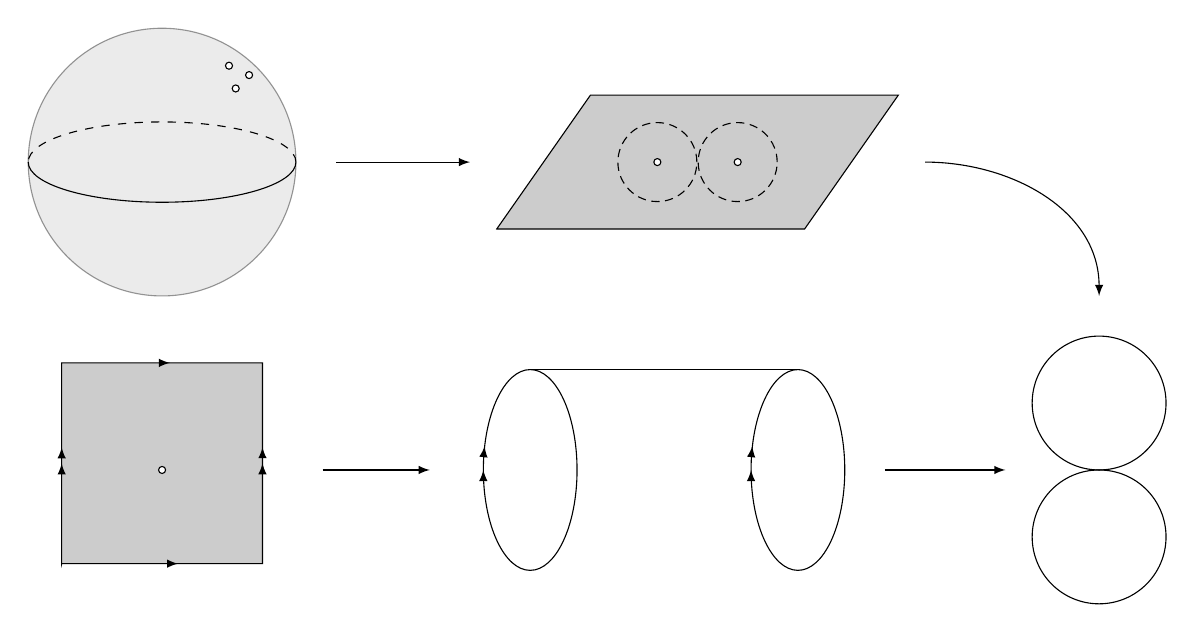
\begin{tikzpicture}[%
        every edge/.style = {%
            draw = black
        },
        scale = 1.7,
        > = latex
    ]

        % Draw a sphere and puncture it with three holes.
        \draw[fill = gray!40, opacity = 0.4] (0.0, 0.0) circle (1cm);
        \draw[fill = white] (0.55, 0.55) circle (0.75pt);
        \draw[fill = white] (0.65, 0.65) circle (0.75pt);
        \draw[fill = white] (0.5, 0.72) circle (0.75pt);

        % Equatorial arcs for the sphere to give it a 3D look.
        \draw (-1.0, 0.0) arc (180:360:1.0 and 0.3);
        \draw[dashed] (1.0, 0.0) arc (0:180:1.0 and 0.3);

        % Arrow transitioning to the next drawing.
        \draw[->] (1.3, 0.0) to (2.3, 0.0);

        % Draw a twice-punctured plane.
        \draw[fill = gray!40]
            (2.5, -0.5) to (3.2, 0.5) to (5.5, 0.5) to (4.8, -0.5) to cycle;
        \draw[fill = white] (3.7, 0.0) circle (0.75pt);
        \draw[fill = white] (4.3, 0.0) circle (0.75pt);
        \draw[densely dashed] (3.7, 0.0) circle (0.295);
        \draw[densely dashed] (4.3, 0.0) circle (0.295);

        % Arc connecting this drawing to the figure-eight curve.
        \draw[->] (5.7, 0.0) to [in = 90, out = 0] (7.0, -1.0);

        % Draw the square representation of the torus.
        \draw[%
            postaction = {decorate},
            decoration = {%
                markings,
                mark = at position 0.145 with \arrow{latex},
                mark = at position 0.375 with \arrow{latex},
                mark = at position 0.395 with \arrow{latex},
                mark = at position 0.615 with \arrowreversed{latex},
                mark = at position 0.855 with \arrowreversed{latex},
                mark = at position 0.875 with \arrowreversed{latex}
            },
            fill = gray!40
        ] (-0.75, -3.0) to (0.75, -3.0) to (0.75, -1.5)
                        to (-0.75, -1.5) to cycle;

        % Puncture the torus.
        \draw[fill = white] (0.0, -2.3) circle (0.75pt);

        % Draw an arrow transitioning to the next figure.
        \draw[->] (1.2, -2.3) to (2.0, -2.3);

        % Draw the skeleton of the torus.
        \draw[%
            postaction = {decorate},
            decoration = {%
                markings,
                mark = at position 0.5 with \arrow{latex},
                mark = at position 0.55 with \arrow{latex}
            }
        ] (3.1,-2.3) arc[%
            start angle = 0,
            delta angle = -360,
            x radius = 0.35,
            y radius = 0.75
        ];

        \draw (2.75, -1.55) to (4.75, -1.55);

        \draw[%
            postaction = {decorate},
            decoration = {%
            markings,
            mark = at position 0.5 with \arrow{latex},
            mark = at position 0.55 with \arrow{latex}
            }
        ] (5.1cm, -2.3cm) arc[%
            start angle = 0,
            delta angle = -360,
            x radius = 0.35,
            y radius = 0.75
        ];

        % Final arrow connecting this to the figure-eight curve.
        \draw[->] (5.4, -2.3) to (6.3, -2.3);

        % Draw the figure eight.
        \draw (7.0, -1.8) circle (0.5);
        \draw (7.0, -2.8) circle (0.5);
    \end{tikzpicture}
\end{document}
